\chapter{光円錐、測地線、シュヴァルツシルト地平線}

地平線問題は、特殊相対性理論にすでに存在する区別から始まる。近接する二つの事象は、時間的、空間的、または光的な方向に隔てられていることがある。曲率はこの分類を廃止しない。曲率は光円錐を局所的な対象とし、各事象で異なるものとし、計量そのものを動力学的にする。ひとたび計量が分かれば、自由落下する粒子の運動は、平坦な時空における自由な相対論的粒子を記述するのと同じ固有時間の原理から従う。

われわれはこの原理を二度用いる。まず、弱い場においてニュートン運動を再現しなければならない。次に、それをシュヴァルツシルト計量に適用する。そこでは、時間、動径距離、速度の意味が予想外に微妙になる。

\section{時間的、空間的、光的区間}

平坦な時空において、\(c=1\) のもとで、固有時間要素は
\begin{equation}
d\tau^2=dt^2-dx^2-dy^2-dz^2.
\label{eq:l5-minkowski-proper-time}
\end{equation}
非相対論的近似が近いときはいつでも、\(c\) を復元することは有用である：
\begin{equation}
d\tau^2
=dt^2-\frac{dx^2+dy^2+dz^2}{c^2}.
\label{eq:l5-minkowski-c}
\end{equation}
表記 \(d\tau^2\) は右辺が正であることを保証しない。その符号が変位を分類する：
\begin{align}
d\tau^2>0
&\quad\Longleftrightarrow\quad \text{time-like},\\
d\tau^2=0
&\quad\Longleftrightarrow\quad \text{light-like},\\
d\tau^2<0
&\quad\Longleftrightarrow\quad \text{space-like}.
\end{align}
空間的変位に対しては、正の固有距離を定義するのが便利である
\begin{equation}
ds^2=-d\tau^2
=dx^2+dy^2+dz^2-dt^2
\qquad(c=1).
\label{eq:l5-proper-distance}
\end{equation}

光円錐はこれら三つの可能性を組織する。その表面、すなわち内部を満たすものではなく、光的な方向から成る。時間的な方向は円錐の内側にあり、空間的な方向は外側にある。上半分と下半分は未来光円錐と過去光円錐を表す。

\begin{figure}[htbp]
\centering
\includegraphics[width=0.82\textwidth]{lecture_05_figure_02.png}
\caption{黒板に組み立てられた固有時間、固有距離、因果円錐。光線は円錐そのものを占め、内部は時間的であり、外部は空間的である。}
\lectureframe{00:05:44}
\end{figure}

\begin{figure}[htbp]
\centering
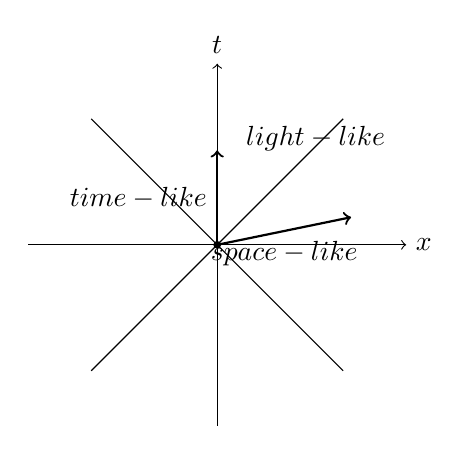
\begin{tikzpicture}[scale=1.0]
\draw[->] (0,-2.3) -- (0,2.3) node[above] {\(t\)};
\draw[->] (-2.4,0) -- (2.4,0) node[right] {\(x\)};
\draw (-1.6,1.6) -- (0,0) -- (1.6,1.6);
\draw (-1.6,-1.6) -- (0,0) -- (1.6,-1.6);
\fill (0,0) circle (1.4pt);
\draw[->,thick] (0,0) -- (0,1.2)
  node[midway,left] {\(\text{time-like}\)};
\draw[->,thick] (0,0) -- (1.7,0.35)
  node[midway,below] {\(\text{space-like}\)};
\node at (1.25,1.35) {\(\text{light-like}\)};
\end{tikzpicture}
\caption{二次元時空断面における因果的分類。}
\end{figure}

これらの区間は操作的である。固有時間とは、時間的世界線に沿って運ばれた時計が示すものである。固有距離とは、適切な一組の物差しが空間的に隔てられた事象の間で測るものである。それらは単に二次形式における符号の名前ではない。

\section{ローレンツ計量の符号と各事象における円錐}

mostly-plus テンソル規約を用いると、平坦計量の成分は
\begin{equation}
\eta_{\mu\nu}=\operatorname{diag}(-1,1,1,1),
\label{eq:l5-eta}
\end{equation}
および
\begin{equation}
d\tau^2=-\eta_{\mu\nu}\,dx^\mu dx^\nu.
\label{eq:l5-proper-time-eta}
\end{equation}
である。表示された行列は、一つの特に単純な基底における二階テンソルの表現である。その不変な特徴はその符号数である：一つの負方向と三つの正方向、
\begin{equation}
\operatorname{signature}(\eta)=(-,+,+,+).
\label{eq:l5-lorentz-signature}
\end{equation}
二つの負符号をもつ計量は二つの時間的方向をもつであろう。そのような符号数は数学的に研究できるが、それらはここで仮定される時空を記述しない。

曲がった時空では成分が変化する：
\begin{equation}
g_{\mu\nu}=g_{\mu\nu}(x).
\label{eq:l5-position-metric}
\end{equation}
各事象において、計量は依然としてローレンツ符号数をもたなければならない。したがって、各事象はそれ自身の時間的方向、光的境界、空間的方向をもつ。座標による図は、点から点へと円錐が傾いたり潰れたりして見えるかもしれないが、因果的分類は保たれる。

\begin{figure}[htbp]
\centering
\includegraphics[width=0.86\textwidth]{lecture_05_figure_03.png}
\caption{位置に依存する計量 \(g_{\mu\nu}(x)\)、因果的ラベル、および局所光円錐のスケッチ。}
\lectureframe{00:09:41}
\end{figure}

\begin{figure}[htbp]
\centering
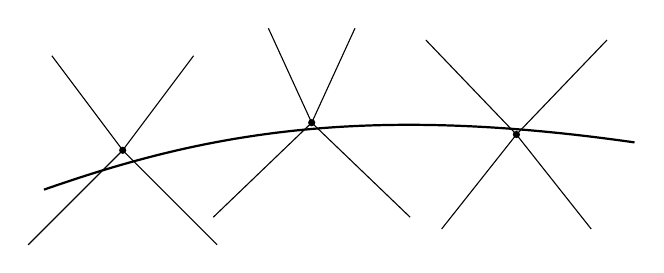
\begin{tikzpicture}[scale=1.0]
\draw[thick] (-4,-0.5) .. controls (-2,0.2) and (0,0.6) .. (3.5,0.1);
\foreach \x/\y/\a/\b in {-3/0/0.9/1.2, -0.6/0.35/0.55/1.25,
                          2.0/0.2/1.15/0.95} {
  \fill (\x,\y) circle (1.3pt);
  \draw (\x,\y) -- ++(-\a,1.2);
  \draw (\x,\y) -- ++(\a,1.2);
  \draw (\x,\y) -- ++(-\b,-1.2);
  \draw (\x,\y) -- ++(\b,-1.2);
}
\end{tikzpicture}
\caption{隣接する局所円錐。どのベクトルが時間的、光的、または空間的であるかを変えることなく、それらの座標上の形は変化しうる。}
\end{figure}

\begin{classroomqa}
\audiencequestion{単一の負の固有値は一つの唯一の時間方向を選び出すのか。}
\lecturerresponse{表示された行列を対角化する基底は一つの負の基底方向をもつが、それは優先的な観測者や唯一の物理的矢印を選び出すものではない。ローレンツ変換は時間座標を空間座標と混ぜ合わせ、円錐の内側にあるすべてのベクトルは時間的である。不変な対象は、円錐と、一つのマイナス、三つのプラスの符号数とを合わせたものであり、一つの特別な時間的ベクトルではない。
\lecturetimestamp{00:12:17--00:17:24}}
\end{classroomqa}

\begin{classroomqa}
\audiencequestion{なぜ局所円錐の二つの図が異なる形をもちうるのか。}
\lecturerresponse{座標は図を変えうる。たとえば、\(x\) を再スケールされた座標で置き換えると、光線に割り当てられる数値的な傾きが変わり、したがって円錐はより狭くまたはより広く見える。より一般的な座標はそれを傾けうる。同じ事象と同じ因果関係が表現されているのである。曲がった時空では、異なる事象における円錐はまた異なる接空間に属するので、それらの比較には計量と輸送規則が必要である。
\lecturetimestamp{00:13:37--00:15:59}}
\end{classroomqa}

\section{変分問題としての測地線}

自由に運動する粒子は時空の測地線に従う。微分形式では、アフィンパラメータ\(\lambda\)を用いて
\begin{equation}
\frac{d^2x^\mu}{d\lambda^2}
+\Gamma^\mu{}_{\rho\sigma}
\frac{dx^\rho}{d\lambda}
\frac{dx^\sigma}{d\lambda}=0.
\label{eq:l5-geodesic}
\end{equation}
接続は、粒子が運動するにつれて接ベクトルがそれ自身と平行であり続ける方法を教える。

しばしば計算がより容易な第二の定式化がある。計量\(g_{mn}\)をもつリーマン空間において、曲線の長さは
\begin{equation}
s=\int ds
=\int\sqrt{g_{mn}\,dx^m dx^n}.
\label{eq:l5-spatial-length}
\end{equation}
測地線は、端点を固定した経路の微小変分の下でこの長さを停留させる。この積分は曲線に沿った微小長さの単なる和であり、そのオイラー--ラグランジュ方程式は、形の上で力の法則に類似した二階微分方程式である。

時間的worldlineに対しては、空間的長さは固有時間で置き換えられる：
\begin{equation}
\tau
=\int\sqrt{-g_{\mu\nu}\,dx^\mu dx^\nu}.
\label{eq:l5-proper-time-functional}
\end{equation}
時間的測地線は\(\tau\)を停留させ、共役点が生じる前の近傍の自由落下経路に対しては局所的に極大とする。\(-m\)を掛けると粒子作用
\begin{equation}
A=-m\tau
=-m\int\sqrt{-g_{\mu\nu}\,dx^\mu dx^\nu}.
\label{eq:l5-particle-action}
\end{equation}
が得られる。したがって同じ経路は\(A=-m\tau\)を局所的に最小化する。停留固有時間と選ばれた作用の符号との区別が、見かけ上の最小対最大の曖昧さを取り除く。

\section{固有時間から通常のラグランジアンへ}

\eqref{eq:l5-particle-action}の作用は幾何学的であるが、力学で用いられる馴染みの形に置くことができる。worldlineを座標\(t\)でパラメータ化し、各微分を\(dt\)で割り、残った因子\(dt\)を平方根の外に引き出す：
\begin{align}
A
&=-m\int\sqrt{-g_{\mu\nu}(x)\,dx^\mu dx^\nu}\\
&=-m\int
\sqrt{-g_{\mu\nu}(x)
\frac{dx^\mu}{dt}\frac{dx^\nu}{dt}}\,dt.
\label{eq:l5-action-t}
\end{align}
時間成分については\(dt/dt=1\)であり、空間成分は通常の座標速度である。したがって
\begin{equation}
\begin{aligned}
A&=\int L\,dt,\\
L&=-m\sqrt{-g_{\mu\nu}(x)\dot x^\mu\dot x^\nu},\\
\dot x^\mu&=\frac{dx^\mu}{dt}.
\end{aligned}
\label{eq:l5-relativistic-lagrangian}
\end{equation}
と書ける。

\begin{figure}[htbp]
\centering
\includegraphics[width=0.88\textwidth]{lecture_05_figure_05.png}
\caption{worldline作用が従来の形\(A=\int L\,dt\)に変換される。}
\lectureframe{00:27:00}
\end{figure}

\begin{figure}[htbp]
\centering
\includegraphics[width=0.88\textwidth]{lecture_05_figure_06.png}
\caption{相対論的ラグランジアンが分離された後の板書状態。}
\lectureframe{00:28:59}
\end{figure}

\begin{classroomqa}
\audiencequestion{この作用の時空指数はギリシャ文字であるべきか？}
\lecturerresponse{はい。ギリシャ文字の指数は時間およびすべての空間座標にわたって走る。ラテン文字の指数は、その区別が有用な場合に空間座標のために取っておいてよい。
\lecturetimestamp{00:25:53--00:26:03}}
\end{classroomqa}

\begin{classroomqa}
\audiencequestion{なぜ平方根の式がラグランジアンと呼ばれるのか？}
\lecturerresponse{作用が\(A=\int L\,dt\)と書かれた後、被積分関数がラグランジアンである。これは単なる定義ではない：その被積分関数を変分するとオイラー--ラグランジュ方程式
\[
\frac{d}{dt}
\left(\frac{\partial L}{\partial\dot x^\mu}\right)
=\frac{\partial L}{\partial x^\mu},
\]
が得られ、これらはパラメータ化が整合的に扱われた後で測地線方程式と等価である。
\lecturetimestamp{00:28:36--00:29:02}}
\end{classroomqa}

質量をもつ粒子に対してworldlineは時間的であるから、平方根の下の量は正である。空間的経路は超光速運動を記述するのであり、通常の質量をもつ粒子の軌道ではない。計量が与えられれば、クリストッフェル記号を計算して\eqref{eq:l5-geodesic}を用いるか、あるいは\eqref{eq:l5-relativistic-lagrangian}にオイラー--ラグランジュを適用することによって、粒子の経路を得ることができる。それらの等価性を示すことは有用な練習である；作用の道筋は通常より短い。

\section{ニュートン極限}

球対称源の外側の弱い静的重力場を考える。平坦時空から始め、\(dt^2\)の係数が1からわずかに異なることを許す：
\begin{equation}
d\tau^2
=\left(1+\frac{2u(\mathbf{x})}{c^2}\right)dt^2
-\frac{d\mathbf{x}^2}{c^2},
\label{eq:l5-weak-metric}
\end{equation}
ここで\(u\)はニュートンポテンシャルになるものである。この仮定は単に名付けるだけでなく、検証されなければならない。

次元をもつ粒子作用は
\begin{equation}
A=-mc^2\int
\sqrt{1+\frac{2u}{c^2}
-\frac{\dot{\mathbf{x}}^{\,2}}{c^2}}\,dt.
\label{eq:l5-weak-action}
\end{equation}
\(u/c^2\)と\(\dot{\mathbf{x}}^{\,2}/c^2\)はともに小さい。それらの一次の寄与を保つと、
\begin{equation}
\sqrt{1+\epsilon}
=1+\frac{\epsilon}{2}+O(\epsilon^2),
\qquad
\epsilon=\frac{2u-\dot{\mathbf{x}}^{\,2}}{c^2},
\end{equation}
により
\begin{align}
L
&=-mc^2
\sqrt{1+\frac{2u-\dot{\mathbf{x}}^{\,2}}{c^2}}\\
&=-mc^2-mu+\frac{m}{2}\dot{\mathbf{x}}^{\,2}\\
&\quad+O\!\left(c^{-2}
 [u^2+u\dot{\mathbf{x}}^{\,2}+\dot{\mathbf{x}}^{\,4}]\right).
\label{eq:l5-newton-expansion}
\end{align}
が得られる。定数の静止エネルギー項は運動方程式に影響しない。残るのは
\begin{equation}
L_{\mathrm{nr}}
=\frac{m}{2}\dot{\mathbf{x}}^{\,2}-m u(\mathbf{x}),
\label{eq:l5-newton-lagrangian}
\end{equation}
であり、したがって
\begin{equation}
m\ddot{\mathbf{x}}=-m\boldsymbol{\nabla}u.
\label{eq:l5-newton-equation}
\end{equation}
である。試験質量は、普遍的自由落下に対してそうでなければならないように、相殺される。ポテンシャルエネルギーは\(m u\)であり、一方加速度は\(m\)に依存しない。

したがって我々は主要な弱場の関係
\begin{equation}
g_{00}=1+\frac{2u}{c^2}+O(c^{-4}).
\label{eq:l5-g00-newton}
\end{equation}
を同定した。球対称質量\(M\)の外側では、
\begin{equation}
u(r)=-\frac{GM}{r},
\qquad
g_{00}=1-\frac{2GM}{rc^2}+O(c^{-4}).
\label{eq:l5-g00-spherical}
\end{equation}
である。これは時間成分への最初の補正を決定する。それはまだ完全な強場計量を決定しない。

\section{球座標と最初のシュヴァルツシルトの推測}

球座標は中心源に対して自然である。この講義では\(\theta\)を極からではなく赤道面から測るので、その角度線素は
\begin{equation}
d\Omega^2=d\theta^2+\cos^2\theta\,d\phi^2.
\label{eq:l5-angular-metric}
\end{equation}
である。この規約では、
\begin{equation}
d\mathbf{x}^2=dr^2+r^2d\Omega^2.
\label{eq:l5-flat-spherical}
\end{equation}
である。この緯度のような\(\theta\)の選択に物理的に依存するものは何もない；より一般的な極角を用いれば\(\cos^2\theta\)は
\(\sin^2\theta\)に置き換えられるであろう。

ニュートン的な時間係数を挿入しつつ空間計量を平坦なままにすると、最初の推測
\begin{equation}
\begin{aligned}
d\tau^2
&=\left(1-\frac{r_s}{r}\right)dt^2
-\frac{1}{c^2}\left(dr^2+r^2d\Omega^2\right),\\
r_s&=\frac{2GM}{c^2}.
\end{aligned}
\label{eq:l5-naive-schwarzschild}
\end{equation}
が得られる。これは厳密な答えではあり得ない。\(r<r_s\) では、\(dt^2\) の係数は符号を変えるが、固有時規約ではすべての空間係数は負のままである。計量はその一時間・三空間の符号数（signature）を失うことになる。

真空場の方程式が、必要とされる動径方向の係数を与える：
\begin{equation}
\boxed{
d\tau^2
=\left(1-\frac{r_s}{r}\right)dt^2
-\frac{dr^2}{c^2\left(1-r_s/r\right)}
-\frac{r^2}{c^2}d\Omega^2.
}
\label{eq:l5-schwarzschild}
\end{equation}
これが外部シュヴァルツシルト計量である。\(r\) が \(r_s\) を通過するとき、\(t\) と \(r\) の係数はともに符号を変え、ローレンツ符号数が保たれる。シュヴァルツシルト座標では、動径座標は内部で時間的になり、座標 \(t\) は空間的になる。この入れ替わりは、事象の地平面における座標チャートの破綻を示すものであり、時空幾何の局所的な破綻ではない。

\begin{classroomqa}
\audiencequestion{落下する物体が地平面を横切るのにどれだけの時間がかかるか。}
\lecturerresponse{遠方の観測者が用いるシュヴァルツシルト座標 \(t\) で測ると、横切りは無限の時間に押しやられる。落下する物体の時計の固有時で測ると、それは有限の時間で起こる。これらの時計の区別が、地平面をめぐる中心的な難問である。
\lecturetimestamp{00:54:45--00:55:35}}
\end{classroomqa}

\begin{classroomqa}
\audiencequestion{なぜ計量の他の部分ではなく、動径方向の係数を変更するのか。}
\lecturerresponse{計量はローレンツ符号数を保たねばならず、球対称性が動径方向を角度方向の球面から区別し、真空場の方程式が逆数の因子を正確に決定する。符号数だけがどこを探すべきかの動機を与え、アインシュタイン方程式が厳密な結果を与える。
\lecturetimestamp{00:55:35--00:56:01}}
\end{classroomqa}

地球の場合、\(r_s\) はわずかセンチメートル程度であり、物質体の深部にある。外部真空計量はそこでは有効でないため、地球はシュヴァルツシルト地平面を持たない。内部解が物質内部でそれを置き換え、表面で接続しなければならない。

\begin{classroomqa}
\audiencequestion{もし \(t\) と \(r\) が座標の役割を交換するなら、普通の時計はどうなるのか。}
\lecturerresponse{時計は時間的世界的線上で固有時を測り続ける。選んだ座標が扱いにくくなったことを時計は知らない。正則な自由落下座標系は、地平面を通して滑らかな局所幾何と通常の局所的な光の伝播を示す。
\lecturetimestamp{00:56:35--00:57:50}}
\end{classroomqa}

\subsection{動径方向の補正がニュートンの方程式に現れなかった理由}

厳密な計量は、ポテンシャルの一次の段階ですでに動径方向の係数を変える：
\begin{equation}
\frac{1}{1-r_s/r}
=1+\frac{r_s}{r}
+O\!\left(\frac{r_s^2}{r^2}\right)
=1-\frac{2u}{c^2}+O(c^{-4}).
\label{eq:l5-radial-expansion}
\end{equation}
ニュートン的な導出でその変化を無視することがなぜ正当化されたのか。粒子作用の内部でそれは \(\dot r^2/c^2\) に掛かる。したがってその最初の補正は
\begin{equation}
\frac{u\,\dot r^2}{c^4},
\end{equation}
に比例し、これは
\eqref{eq:l5-newton-expansion}
で保持された次数を超えている。動径方向の補正は低速運動のニュートン的検証では無視できるが、相対論的運動や地平面の近くでは決定的になる。これは有用な警告である：ある近似にとって小さすぎる項が、別の近似では関心のある現象を支配することがある。

\section{シュヴァルツシルト時間における動径方向の落下}

\(c=1\) と置き、まず動径方向の運動を調べる。円軌道も重要であるが、それには角度方向の項が必要であり、後回しにする。動径方向の運動は軌道というよりも源へ向かう直接の衝突であり、最小限の代数で地平面の振る舞いを露わにする。

\begin{classroomqa}
\audiencequestion{動径方向の速度には誰の時間が現れるのか。}
\lecturerresponse{下のドットは、シュヴァルツシルト座標時間 \(t\) に関する微分を意味する。これは遠方の静的観測者に規格化された時間である。落下する観測者の腕時計は固有時 \(\tau\) を測る。両者を混同すると、座標に関する記述が誤った局所的な記述に変わってしまう。
\lecturetimestamp{01:04:03--01:04:47}}
\end{classroomqa}

\(d\Omega=0\) に対し、
\begin{equation}
a(r)=1-\frac{r_s}{r}.
\label{eq:l5-a-def}
\end{equation}
と定義する。動径方向の計量とラグランジアンは
\begin{align}
d\tau^2&=a\,dt^2-\frac{dr^2}{a},\\
L&=-m\sqrt{a-\frac{\dot r^2}{a}},
\qquad
\dot r=\frac{dr}{dt}.
\label{eq:l5-radial-lagrangian}
\end{align}
である。\(L\) は \(t\) に陽に依存しないので、そのハミルトニアンは保存される。動径方向の運動量は
\begin{equation}
p_r=\frac{\partial L}{\partial\dot r}
=\frac{m\dot r}{a\sqrt{a-\dot r^2/a}},
\label{eq:l5-radial-momentum}
\end{equation}
であり、
\begin{align}
H
&=p_r\dot r-L\\
&=\frac{ma}{\sqrt{a-\dot r^2/a}}
=E.
\label{eq:l5-radial-energy}
\end{align}
である。座標速度について解くと
\begin{equation}
\boxed{
\dot r^2
=a^2\left(1-\frac{m^2}{E^2}a\right).
}
\label{eq:l5-radial-velocity}
\end{equation}
が得られる。板書の計算ではいくつかの中間的な代数形を検討するが、枠で囲まれた式が整合する結果である。

\(r\) が \(r_s\) に近づくにつれ、\(a(r)\) はゼロに近づき、括弧内の因子は1に近づく。したがって、内向きの粒子に対して
\begin{equation}
\frac{dr}{dt}
\sim -\left(1-\frac{r_s}{r}\right)
\longrightarrow 0
\qquad(r\longrightarrow r_s^+)
\label{eq:l5-infall-freeze}
\end{equation}
となる。シュヴァルツシルト時間では、粒子は地平面のすぐ外側で減速し凍りつくように見える。

\begin{classroomqa}
\audiencequestion{\(dr/dt\)の値が減少することは、重力が斥力になったという意味だろうか。}
\lecturerresponse{いいえ。粒子は局所的に外へ押し出されているのではない。座標\(t\)は、この横断を記述するのにはますます不適切になるため、単位\(t\)あたりの動径方向の進みはゼロに近づく。自由落下する世界線に沿った固有加速度はゼロのままであり、事象の地平面には有限の固有時間で到達する。
\lecturetimestamp{01:14:18--01:16:38}}
\end{classroomqa}

実際、地平面の近くでは
\begin{equation}
\frac{dt}{dr}
\sim-\frac{1}{1-r_s/r}
=-\frac{r}{r-r_s}.
\end{equation}
その積分は対数的に発散する。これは、落下する時計の読みが無限になることを意味することなく、シュヴァルツシルト時間が無限であるという主張を証明している。

\section{動径方向の光線}

光は同じ計算の最も短い版を与える。動径方向のヌル光線に対して、
\begin{equation}
d\tau^2
=a\,dt^2-\frac{dr^2}{a}=0.
\end{equation}
したがって
\begin{equation}
\boxed{
\frac{dr}{dt}
=\pm a(r)
=\pm\left(1-\frac{r_s}{r}\right).
}
\label{eq:l5-radial-light}
\end{equation}
プラス符号は外向きの光線を表し、マイナス符号は内向きの光線を表す。どちらの座標速度も地平面でゼロに近づく。

\begin{classroomqa}
\audiencequestion{この式は光源から遠く離れるとどのような速度を与えるか。}
\lecturerresponse{\(r\)が無限大に近づくと、\(a(r)\)は1に近づくので、\(dr/dt\)は\(\pm1\)に近づき、単位を戻せば\(\pm c\)に近づく。
\lecturetimestamp{01:21:01--01:21:29}}
\end{classroomqa}

一般相対性理論はしばしばこのようなものである。原理は数行に収まるが、座標と計算は複雑になっていく。式\eqref{eq:l5-radial-light}は単純だが、\(r_s\)の近くでそれがゼロになることを解釈するには注意が必要である。それは座標速度であり、局所慣性観測者が測定する速度ではない。

\section{遠方の観測者が見るもの}

\begin{classroomqa}
\audiencequestion{地平面の近くで放出された光は脱出できるか、そしてそれはホーキング放射か。}
\lecturerresponse{地平面のすぐ外側で放出された外向きの古典的光線は外へ進むことができるが、そのシュヴァルツシルト座標速度は極めて小さく始まり、信号が無限遠に到達するのは甚だしい遅延と赤方偏移の後になってからである。地平面上の光線はこれらの座標では地平面上にとどまり、内側の光線は脱出できない。ホーキング放射は外部の幾何に関連する量子場の効果であり、内側から古典的な光線が這い上がってくるものではなく、本計算によって導出されるものでもない。
\lecturetimestamp{01:22:08--01:24:28}}
\end{classroomqa}

\begin{classroomqa}
\audiencequestion{光子がほとんど静止して見えるなら、質量を持つように見え始めるのか。}
\lecturerresponse{いいえ。自由落下する局所観測者は常に光子が\(c\)で運動していると測定する。座標比\(dr/dt\)だけがゼロに近づく。質量、ヌル性、光の局所速度は、悪い座標チャートによって変わることはない。
\lecturetimestamp{01:24:31--01:25:26}}
\end{classroomqa}

ここで用いたシュヴァルツシルト表式は真空の外部解である。恒星、惑星、または崩壊する雲は、それと接続されなければならない異なる内部計量を持つ。物質表面が\(r_s\)の外側にとどまるなら、地球が莫大な余裕をもってそうであるように、外部座標の地平面は、真空の式を物質を通して延長できる領域の外側にある。天体がそのシュヴァルツシルト半径の内側へ崩壊するなら、地平面は物理的時空の一部となる。

\begin{classroomqa}
\audiencequestion{外部の観測者が物質の横断を決して見ないなら、ブラックホールはどうして形成され、または成長しうるのか。}
\lecturerresponse{その前提は、シュヴァルツシルト時間を地平面における大域的な物理的時計であるかのように用いている。したがってブラックホールは決して成長しえないという結論は、もっともらしく聞こえるが誤りである。完全な答えには、正則な地平面横断座標と崩壊の大域的因果幾何が必要であり、その解決はこの講義の次の段階に先送りされる。
\lecturetimestamp{01:27:57--01:29:36}}
\end{classroomqa}

\begin{classroomqa}
\audiencequestion{地平面へ落下する車に対して、レーダー銃は何を報告するだろうか。}
\lecturerresponse{座標速度は車が落下するにつれてまず増加し、その後反転してゼロに向かって減少する。後から送られたレーダーパルスは依然として地平面の外側で車を捉えることができるが、往復には次第に長い時間がかかる。返ってくる信号はますます赤方偏移し、像は\(r_s\)の近くで遅くなり圧縮されて見える。これは運転者が経験するものの信頼できる局所的描像ではない。運転者は有限の固有時間で横断する。
\lecturetimestamp{01:29:39--01:32:14}}
\end{classroomqa}

\begin{classroomqa}
\audiencequestion{光の速度は特殊相対性理論においてのみ一定なのか。}
\lecturerresponse{一般相対性理論においても、あらゆる局所慣性系で一定である。局所的な時計と物差しを伴って落下する観測者は、近くの光子を\(c\)で測定する。\(dr/dt\)のような座標速度は、\(r\)と\(t\)が時空全体にわたる一つの局所慣性実験室の読みではないために変わりうる。
\lecturetimestamp{01:32:20--01:34:20}}
\end{classroomqa}

\section{シュヴァルツシルト計算を超える問い}

\begin{classroomqa}
\audiencequestion{重力を他の力と統一するとは、いったい何を意味しうるのだろうか。}
\lecturerresponse{一つの幾何学的な可能性は、時空を追加のコンパクトな方向で拡大することである。そのとき、高次元計量の成分は4次元においてゲージ場やスカラー場として現れうるし、余分な方向の運動量は電荷として現れうる。これはKaluza--Kleinのアイデアに関連する構造的な示唆であって、本講義における完成した統一ではない。
\lecturetimestamp{01:34:22--01:36:08}}
\end{classroomqa}

\begin{classroomqa}
\audiencequestion{異なる領域や宇宙が異なる計量の符号数を持ちうるだろうか。}
\lecturerresponse{古典的一般相対性理論は、通常、非退化なローレンツ符号数を固定する。それを変えるには、計量が退化した配置を通過する必要があり、そこでは標準的な古典的記述が破綻する。量子重力はより広い言語を強いるかもしれないが、物理的な符号数変化領域を予言する確立された理論はここにはない。
\lecturetimestamp{01:36:08--01:38:08}}
\end{classroomqa}

\begin{classroomqa}
\audiencequestion{第一次世界大戦中に従軍しながら、Schwarzschildはどのようにしてこの解を見つけたのか。}
\lecturerresponse{授業でなされた指摘は、歴史的であると同時に人間的でもある。Schwarzschildは天文学者であり、きわめて卓越した数学者でもあり、Einsteinの新しい方程式に取り組むことは、戦時従軍のさなかにおける知的避難所を提供したのである。
\lecturetimestamp{01:38:11--01:39:02}}
\end{classroomqa}

中心的な教訓は、今や先へ持ち運ぶのに十分鋭くなっている。計量は因果錐と自由運動の両方を決定する。その弱場の時間成分はNewtonのポテンシャルを含み、一方その厳密なSchwarzschildの形は\(r=r_s\)に座標地平線を与える。Schwarzschild時間は横断を無限大に引き伸ばすが、落下する観測者の固有時間はそうしない。この対比を大域的に解決し、凍りついた遠方の像にもかかわらずブラックホールがどのように形成されるかを説明することが、次の問題である。
